\chapter{Modeling Photovoltaics}

% TODO: intro paragraph for chapter 1
\todo{Insert intro paragraph on the focus of this chapter, as well as the a
short discussion of the following sections.}

\newpage
\section{Three Parameter Solar Cell Model}

The most basic model of a solar cell is the three parameter model, or single
diode model. It consists of a constant current source that produces \ac{IPV},
and a diode that consumes part of \ac{IPV} in the form of \ac{ID}. The
remaining \ac{I} is left to be sunk into the \ac{RL}. We consider this model
ideal, since it does not incorporate cell losses in the form of \ac{RS} and
\ac{RSH}. It is assumed that the series resistance is zero or short circuit and
the shunt resistance is infinite or open circuit. This is addressed in the five
parameter and seven parameter models.

The load current \ac*{I} in Figure~\ref{fig:single_diode_model} can be
represented as a function of the photocurrent \ac*{IPV} and the dark current
\ac*{ID}, shown in Equation~\ref{eq:cell_output_current_1}.

\begin{figure}[h]
    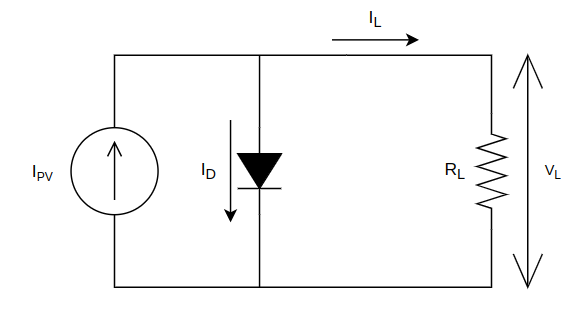
\includegraphics[width=\textwidth]{solar_cell_three_parameter_model.png}
    \caption{Three Parameter, or Single Diode Model of a Solar Cell}
    \label{fig:single_diode_model}
\end{figure}

\begin{equation}
    I = I_{PV} - I_D~A
    \label{eq:cell_output_current_1}
\end{equation}

\subsection*{Photocurrent and Short Circuit Current}

On a fundamental level, we can define the photocurrent \ac{IPV} as a function of
the photons incident upon the surface of the solar cell and the spectral
response of the solar cell. This is demonstrated in
Equation~\ref{eq:cell_photocurrent}. A bulleted explanation of this equation
oriented for the layman is as follows:

\begin{equation}
    I_{PV} = qA\int_{}{}b_s(E)QE(E)dE~A
    \label{eq:cell_photocurrent}
\end{equation}

\begin{itemize}
    \item Incident light hits the solar cell over a given spectrum of energy
    levels (denoted either in $eV$ or in $nm$) (see
    Figure~\ref{fig:maxeon_gen_iii_cell_spectral_response}).
    \item Incident light at each discrete energy level has an \ac{BS}, otherwise
    known as intensity.
    \item The solar cell has a given \ac{QE} at each energy level, which is the
    probability that an incident photon of \ac{E} delivers one electron to the
    external circuit.
    \item Integrating the product of the photon flux density \ac{BS} and quantum
    efficiency \ac{QE} (then multiplied by the \ac{Q} and the cell \ac{A})
    provides the photocurrent \ac{IPV}.
\end{itemize}

\begin{figure}[h]
    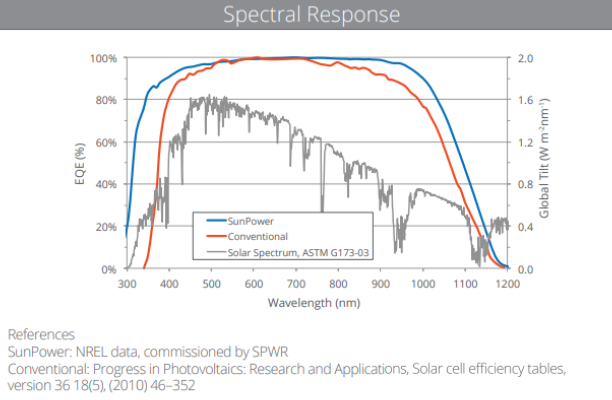
\includegraphics[width=\textwidth]{maxeon_gen_iii_cell_spectral_response.png}
    \caption{Maxeon Gen III Cell Spectral Response}
    \label{fig:maxeon_gen_iii_cell_spectral_response}
\end{figure}

Solar cell manufacturers may provide a spectral response chart showing the
quantum efficiency over the useful solar spectrum (as seen in
Figure~\ref{fig:maxeon_gen_iii_cell_spectral_response}), but will generally just
provide the \ac{ISC} at \ac{STC} ($1000$ $Wm^-2$, $AM$ $1.5G$, $25$ $C$).

As it turns out, the photocurrent \ac{IPV} can generally be approximated as the
short circuit current \ac{ISC}.

\begin{equation}
    I_{PV} = I_{SC}~A
    \label{eq:cell_photocurrent_simplified}
\end{equation}

We'll discuss in a further section that Cubas et al.~\cite{cubas_et_al} defines
the photocurrent as a ratio of the series and shunt resistance in addition to
the short circuit current. However, in most cases the empirical value of
\ac{ISC} does not differ from Equation~\ref{eq:cell_photocurrent_simplified}.

\subsection*{Dark Current}

The dark current \ac{ID} comprises of the interesting and critical parameters of
the three parameter model shown in
Equation~\ref{eq:cell_dark_current_simplified}; it contains the \ac{I0} and an
exponential. The exponential is a function of \ac{TC} and \ac{V} applied across
the cell. The term \ac{VT} which encapsulates the \ac{TC} dependence describes
the voltage across the P-N junction of the diode in the model: at \ac{STC} this
is typically $26$ $mV$. It is defined by Equation~\ref{eq:cell_thermal_voltage}.

\begin{equation}
    I_D = I_0[exp(\frac{V}{V_T}) - 1]~A
    \label{eq:cell_dark_current_simplified}
\end{equation}

\begin{equation}
    V_T = \frac{k_BT_C}{q}~V
    \label{eq:cell_thermal_voltage}
\end{equation}

\subsection*{Dark Saturation Current}

The dark saturation current \ac{I0} has two potential derivations.
Generally, the three parameter model, (see Baig et al.~\cite{baig_et_al},
MacAlpine et Brandemuehl~\cite{macalpine_et_brandemuehl}, Rusirawan et
Farkas~\cite{rusirawan_et_farkas}, and others) define \ac{I0} as in
Figure~\ref{eq:cell_dark_saturation_current_1}; where the diode current is a
function of the cell temperature and the energy bandgap in relation to a
several reference parameters at \ac{STC}. These terms cancel each other out in
the exponential, so the eventual subtraction is unitless.

\begin{equation}
    I_0 = I_{0,ref}(\frac{T_C}{T_{C,ref}})^3exp(\frac{E_{G,ref}}{k_BT_{C,ref}} - \frac{E_G}{k_BT_C})~A
    \label{eq:cell_dark_saturation_current_1}
\end{equation}

On the other hand, we can derive the \ac{I0} numerically, given \ac{ISC} and
\ac{VOC}, by setting the cell at open circuit: at open circuit, there is no load
therefore the cell is at \ac{VOC}. This is shown by
Figure~\ref{eq:cell_dark_saturation_current_2}.

\begin{equation}
    I_0 = I_{SC}[exp(\frac{V_{OC}}{V_T}) - 1]^{-1}~A
    \label{eq:cell_dark_saturation_current_2}
\end{equation}

These two models of the reverse saturation current will be explored further in
this major section.

\subsection*{Short Circuit Current}

Finally, for the three parameter model, we derive the dependence of \ac{ISC}
and \ac{VOC} on irradiance and temperature before establishing the final
derivation of Equation~\ref{eq:cell_output_current_1}.

It is known that for the short circuit current, there is a large positive
correlation with irradiance and a small positive correlation with temperature,
shown in Figures~\ref{fig:cell_temperature_dependence}
and~\ref{fig:cell_irradiance_dependence}.

\begin{figure}[h]
    \centering
    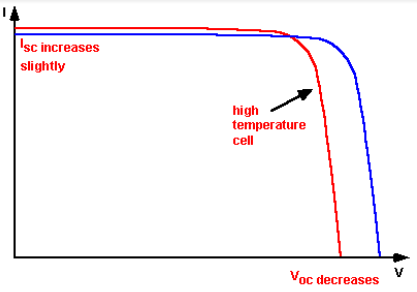
\includegraphics[width=0.7\linewidth]{cell_temperature_dependence.png}
    \caption{Solar Cell Temperature Dependence}
    \label{fig:cell_temperature_dependence}
\end{figure}

\begin{figure}[h]
    \centering
    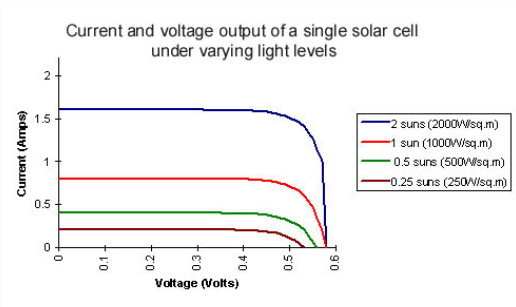
\includegraphics[width=0.9\linewidth]{cell_irradiance_dependence.png}
    \caption{Solar Cell Irradiance Dependence}
    \label{fig:cell_irradiance_dependence}
\end{figure}

The dependence of irradiance on short circuit current can be modeled as linearly
proportional to the light incident upon the solar cell over the reference
irradiance. This makes intuitive sense: given half the available light (assuming
the distribution of light across the spectrum is consistent), the solar cell
will only be able to capture half the maximum available power. Chegaar et
al.~\cite{chegaar_et_al} proposes this relationship as
Equation~\ref{eq:cell_short_circuit_current_1}, where the short circuit current
is a function of \ac{KE} and \ac{G} in $Wm^{-2}$.

\begin{equation}
    I_{SC}(G) = K_EG~A
    \label{eq:cell_short_circuit_current_1}
\end{equation}

Equation~\ref{eq:cell_short_circuit_current_1} can be easily reworked where the
constant \ac{KE} is now based on a reference short circuit current and
irradiance, preferably at \ac{STC}. This forms
Equation~\ref{eq:cell_short_circuit_current_2}, which is the same form used by
Baig et al.~\cite{baig_et_al}.

\begin{equation}
    I_{SC}(G) = I_{SC,ref}\frac{G}{G_{ref}}~A
    \label{eq:cell_short_circuit_current_2}
\end{equation}

Hishikawa et al.~\cite{hishikawa_et_al} proposes modeling the dependence of
temperature on short circuit current density using a thermal coefficient,
$\alpha$. $\alpha$ is empirically determined given the material composition and
structure of the solar cell; for crystalline silicon solar cells, this is
approximately 0.05\%/K, or 0.0005. Equation~\ref{eq:thermal_coefficient_alpha}
shows how given $\alpha$ the change in temperature affects short circuit current
density and vice versa. Rearranging the equation leads to the derivation
Equation~\ref{eq:cell_short_circuit_current_3}.

\begin{equation}
    \alpha = \frac{1}{I_{SC,ref}}\frac{\Delta I_{SC}}{\Delta T_C} = \frac{1}{I_{SC,ref}}\frac{I_{SC,ref} - I_{SC}}{T_{C,ref} - T_C}
    \label{eq:thermal_coefficient_alpha}
\end{equation}

\begin{equation}
    I_{SC}(T_C) = I_{SC,ref}[1 - \alpha(T_{C,ref} - T_C)]~A
    \label{eq:cell_short_circuit_current_3}
\end{equation}

% TODO: finish up this section.
Interestingly, Rusirawan et Farkas~\cite{rusirawan_et_farkas} and MacAlpine et
Brandemuehl~\cite{macalpine_et_brandemuehl} perform two different variants:
Rusirawan et Farkas models the temperature dependence as a
\todo{Describe the differentiation between these three variants of \ac{ISC}}
\dots, shown in
Equation~\ref{eq:cell_short_circuit_current_4}, and MacAlpine et Brandemuehl
models the temperature dependence as a \dots, shown in
Equation~\ref{eq:cell_short_circuit_current_5}.

\begin{equation}
    I_{SC}(T_C) = I_{SC,ref}+\mu(T_{C,ref} - T_C)~A, where
    \label{eq:cell_short_circuit_current_4}
\end{equation}
\begin{equation}
    \mu = \frac{I_{SC} - I_{SC,ref}}{T_C - T_{C,ref}} = -\alpha
\end{equation}

\begin{equation}
    I_{SC}(T_C) = I_{SC,ref}[I_{SC,ref} + \propto (T_{C,ref} - T_C)]~A
    \label{eq:cell_short_circuit_current_5}
\end{equation}

Combining Equations~\ref{eq:cell_short_circuit_current_2}
and~\ref{eq:cell_short_circuit_current_3} give us
Equation~\ref{eq:cell_short_circuit_current_6}.

\begin{equation}
    I_{SC}(G, T_C) = I_{SC,ref}\frac{G}{G_{ref}}[1 - \alpha(T_{C,ref} - T_C)]~A
    \label{eq:cell_short_circuit_current_6}
\end{equation}

These three models of the short circuit current will also be explored further in
this major section.

\subsection*{Open Circuit Voltage}

Likewise, the open circuit voltage is also a function of temperature and
irradiance. It is known that the open circuit voltage has a medium positive
correlation with irradiance and a medium negative correlation with temperature,
shown back in Figures~\ref{fig:cell_temperature_dependence}
and~\ref{fig:cell_irradiance_dependence}.

Returning to Equation~\ref{eq:cell_dark_saturation_current_2}, in which we
defined the dark saturation current \ac{I0} as a function of the open circuit
voltage \ac{VOC}, we can invert the equation to retrieve the \ac{VOC} parameter,
shown in Equation~\ref{eq:cell_open_circuit_voltage_1}.

\begin{equation}
    V_{OC} = V_T\ln(\frac{I_{SC}}{I_0} + 1)~V
    \label{eq:cell_open_circuit_voltage_1}
\end{equation}

There are three points in this equation that can now be determined. We know from
Equation~\ref{eq:cell_thermal_voltage} that the thermal voltage is dependent on
the cell temperature \ac{TC}. We can also plug in one of the proposed models for
\ac{ISC}. However, we cannot reuse
Equation~\ref{eq:cell_dark_saturation_current_2} because
Equation~\ref{eq:cell_open_circuit_voltage_1} was derived from it! Chegaar et
al.~\cite{chegaar_et_al} simplifies the logarithmic term to form
Equation~\ref{eq:cell_open_circuit_voltage_2}.

\begin{equation}
    V_{OC}(G, T_C) = V_{OC,ref} + V_T(T_C)\ln(\frac{G}{G_{ref}} + 1)~V
    \label{eq:cell_open_circuit_voltage_2}
\end{equation}

This term fits well with the paper’s experimental data, but is not immediately
clear how it models the original term. It also does not properly model
temperature change. Equation~\ref{eq:cell_open_circuit_voltage_3} is a modified
form that implements temperature dependence while retaining irradiance
dependence.

\begin{equation}
    V_{OC}(G, T_C) = V_{OC,ref}[1 - \beta (T_{C,ref} - T_C)]
        + \frac{k_B(T_{C,ref} + T_C/\gamma)}{q}\ln(\frac{G}{G_{ref}})~V
    \label{eq:cell_open_circuit_voltage_3}
\end{equation}

\begin{equation}
    \beta = \frac{1}{V_{OC,ref}}\frac{\Delta V_{OC}}{\Delta T_C}
          = \frac{1}{V_{OC,ref}}\frac{V_{OC,ref} - V_{OC}}{T_{C,ref} - T_C}
    \label{eq:thermal_coefficient_beta}
\end{equation}

Equation~\ref{eq:cell_open_circuit_voltage_3} implements two changes: a linear
constant $\beta$ that represents the open circuit voltage temperature
coefficient and a modifier $T_C/\gamma$. $\beta$ is likewise empirically
determined given the material composition and structure of the solar cell; for
silicon it known to be -0.3\%/K, or 0.003.

% TODO: curve fitting term for V_OC
\todo[inline]{This fits expected data from other papers, but need to test on our setup.}
The modifier is an experimentally determined curve fitting term, and
appropriately models the exponential decrease of \ac{VOC} at low light
conditions. It has an operable range of values between $[1, 100]$, where smaller
values means a wider range of of \ac{VOC} movement at llow light conditions.

\subsection*{Model Summary}

% TODO: phrasing
\todo[inline]{I don't agree with \ac{IPV}, \ac{ID}, and \ac{N} being the "parameters".
It makes more sense for \ac{G}, \ac{TC}, $\alpha$, $\beta$, and $\gamma$ to be
the parameters, since they are actually empirically measured/changed.}
To conclude this major section, let's bring in all the pieces developed by this
model. Firstly, we know that the load current for the single diode solar cell
model is dependent on two primary components: photocurrent source and a dark
current sink. These two components are dependent on a set of intrinsic and
extrinsic factors, namely build quality and uniformity, irradiance, temperature,
and load.

The three parameters in this model are the two components aforementioned plus an
\ac{N}. This factor is between 1 and 2, and is a proxy for cell recombination.

The final model function is presented in
Equation~\ref{eq:cell_output_current_2}.

% I(V, G, T_C) = I_PV - I_D
% I(V, G, T_C) = I_SC - I_0(exp(V/V_T) - 1)
% I(V, G, T_C) = I_SC - I_SC((exp(V_OC/V_T)-1)^-1)(exp(V/V_T) - 1)
% I_SC = I_{SC,ref}\frac{G}{G_{ref}}[1 - \alpha(T_{C,ref} - T_C)]
% V_OC = V_{OC,ref}[1 - \beta (T_{C,ref} - T_C)] + \frac{k_B(T_{C,ref} + T_C/\gamma)}{q}\ln(\frac{G}{G_{ref}})
\begin{equation}
    \begin{split}
        I(V, G, T_C) = &I_{SC,ref}\frac{G}{G_{ref}}[1 - \alpha(T_{C,ref} - T_C)] - \\
        & I_{SC,ref}\frac{G}{G_{ref}}[1 - \alpha(T_{C,ref} - T_C)] \\
        & [exp(\frac{V_{OC,ref}[1 - \beta (T_{C,ref} - T_C)] + \frac{nk_B(T_{C,ref} + T_C/\gamma)}{q}\ln(\frac{G}{G_{ref}})}{\frac{nk_BT_C}{q}}) - 1]^{-1} \\
        & [exp(\frac{V}{\frac{nk_BT_C}{q}}) - 1] A
    \end{split}
    \label{eq:cell_output_current_2}
\end{equation}

\todo[inline]{See https://www.desmos.com/calculator/yp0rhmabkz to play around
with model. Add as figure later on compared to experimental data.}

\newpage
\section{Five Parameter Solar Cell Model}

\newpage
\section{Seven Parameter Solar Cell Model}


\newpage
\section{Evaluating Solar Cell Models}

\subsection*{Solar Cell Dataset}

\todo{Refer to Appendix for testing setup}

\subsection*{Methods to Fit Cells}